\section{Introduction}
\label{sec:intro}

\begin{figure}[t]
\centering
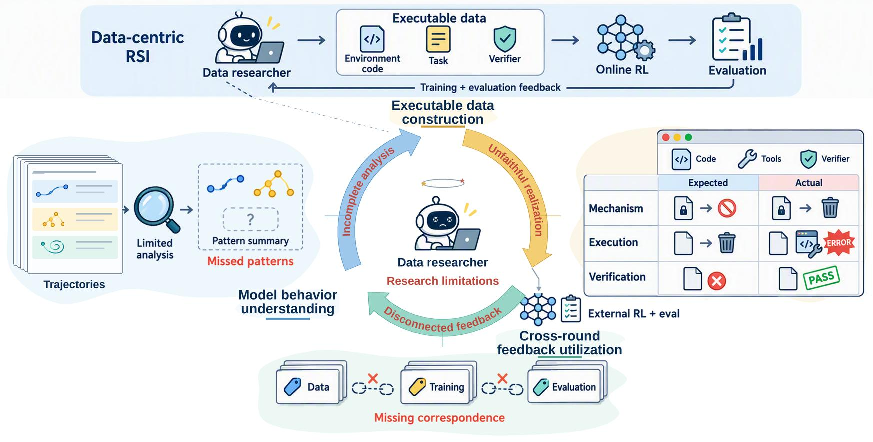
\includegraphics[width=\linewidth]{figures/overview.pdf}
\caption{Data-centric RSI and a typical native-Codex research workflow. \method{} addresses its bottlenecks with traceable analysis, target-grounded generation, and a target-linked environment pool.}
\label{fig:overview}
\end{figure}



Recursive self-improvement (RSI) asks whether AI systems can use evidence from one development cycle to improve the next. MetaRSI\textcolor{magenta}{[CITE: MetaRSI]} distinguishes three writable surfaces for improvement: data, the execution harness, and model parameters. We focus on the interaction between the data and model surfaces, where an agent adapts training data as the learner evolves. Relatedly, RSIBench-Data~\citep{rsibenchdata} studies agents that revise training-data strategies across training runs and reveals a discovery--reliability gap: agents can discover useful strategies but struggle to improve them consistently. This raises a sharper question: when the learner itself changes, can feedback from one training round reliably guide data construction for the next?

We study this question in the context of training agents to use tools more effectively, as tool use is a fundamental capability for modern agents. Training such agents extend beyond generating static samples because training data take the form of executable instances that define state, tool behavior, tasks, and outcome verification. Systems for executable environment synthesis and scaling, including AgentScaler, EnvScaler, ScaleEnv, Agent World Model, and EnvFactory~\citep{agentscaler,envscaler,scaleenv,awm,envfactory}, show that such resources can be constructed automatically. Building on this capability, we study data-centric recursive improvement in a stateful, multi-round online-RL setting, where a target model is iteratively updated using new data produced by a data-researcher agent. Specifically, starting from an empty pool of executable environments, the agent operates in a four-stage loop: analyzing the current target model's behavior, constructing executable training instances, submitting them to a fixed external service for online-RL training and evaluation, and using the resulting training records and evaluation feedback to guide the next round. With each round continuing from the updated model, the training data and target policy evolve together over time. Reliable recursive improvement is therefore not a one-shot data-generation problem: it requires sustaining a coherent data loop as both continue to evolve. Our experiments show that even a modern agent with strong reasoning and coding capabilities (Codex with GPT-6 Astra) struggles to sustain improvement across rounds. The target model's performance often plateaus or regresses, and some runs even end in training collapse.

Based on our experiments and observations, we identify three key stages in closing the data improvement loop and their associated failure modes:

\begin{itemize}
\item \textbf{Model behavior understanding.} \emph{Incomplete analysis} of available traces yields a partial or biased understanding of the target model.

\item \textbf{Cross-round feedback utilization.} \emph{Disconnected feedback} prevents the agent from relating constructed data to realized training experience and subsequent target behavior.

\item \textbf{Executable data construction.} \emph{Unfaithful realization} produces environments that are logically inconsistent or misaligned with the targeted domain or capability.
\end{itemize}

To these ends, we introduce \method{}, a framework that addresses these failure modes through three corresponding components. To see patterns in target model behavior, a \textbf{traceable behavioral map} consolidates evidence across trajectories while preserving links to the source cases. To close the feedback loop across rounds, \textbf{target-conditioned context refinement} organizes relevant data, observed training dynamics, and subsequent evaluation outcomes around each training target. To faithfully realize each training target as executable data, \textbf{iterative environment construction} uses a planning, implementation, and refinement loop to bridge the last mile from target specification to logically consistent and behaviorally aligned environments.
Extensive experiments across four agentic tool-use benchmarks demonstrate the effectiveness of \method{} for multi-round improvement. On Qwen3-4B, \method{} achieves substantial performance gains of $+7.44$, $+16.67$, $+11.11$, and $+13.29$ percentage points on $\tau^2$-Bench, BFCL-v4, ACEBench-Agent, and AppWorld, respectively. Across successive iterations, target model performance with \method{} follows a clear overall upward trend, whereas the same Codex researcher without these mechanisms produces irregular fluctuations with no sustained direction of improvement. Further analyses show that the three proposed designs improve their corresponding stages of the loop by increasing coverage of task requirements and failure mechanisms, improving the quality of realized RL signals, and producing executable environments that are more reliable and better aligned with their training targets.






